\chapter{Untersuchung geeigneter Process Miner}\label{chap:approach}
Um systematisch einen geeigneten Algorithmus zu finden, der automatisiert Regeln aus den Protokolldateien eines Smart Homes extrahiert, soll eine begrenzte Anzahl an Process Mining Verfahren in Testdurchläufen miteinander verglichen werden. 

Die Durchführung der Testreihe soll sich am Leitfaden für Studien im Bereich des Software Enginieering von Runeson und Höst orientieren \cite{runh}. Der Leitfaden klassifiziert Studien zunächst nach ihrer Fragestellung. Es wird unterschieden zwischen erkundenden (\textit{exploratory}), beschreibenden (\textit{descriptive}), erklärenden (\textit{explanatory}) und verbessernden (\textit{improving}) Forschungsfragen. Der Zweck der hier geplanten Testreihe lässt sich als erkundend einordnen, denn es soll festgestellt werden, ob einer der zu untersuchenden Miner überhaupt in der Lage ist, Verhaltensmuster nach dem If This Then That Schema zu modellieren und die Frage beantworten, ob es Vorteile in einem der untersuchten Verfahren gegenüber einem anderen gibt. 
Der Leitfaden für Informationen erkundende Studien umfasst im wesentlichen fünf Schritte: 

\begin{enumerate}
  \item \textbf{Definition der Ziele}: Welche Erkenntnisse sollen gewonnen werden?
  \item \textbf{Vorbereitung}: Welche Mittel oder Daten werden zur Beantwortung der Fragestellung benötigt?
  \item \textbf{Durchführung}: Die gesammelten Daten und Mittel werden genutzt, um die Studie umzusetzen. 
  \item \textbf{Auswertung}: Worauf lassen die Ergebnisse der Studie schließen?
  \item \textbf{Zusammenfassung}: Bericht zur Studie.
\end{enumerate}

Das Ziel wird in Abschnitt \ref{sec:def} und die Vorbereitung zur Durchführung dieser Testreihe  in Abschnitt \ref{sec:prep} beschrieben. Die Durchführung und Auswertung folgt in Abschnitt  \ref{sec:tests}, das Ergebnis in Abschnitt \ref{sec:res}. Dieses Kapitel soll gleichzeitig als Dokumentation der Testreihe dienen.

\section{Ziel und Motivation der Testreihe}\label{sec:def}
Das Ziel der Testreihe ist es festzustellen, ob es Process Mining Verfahren gelingt aus Datensätzen, die aus einem Smart Home stammen, kurze und repetitive Verhaltensmuster zu modellieren. Die Anforderung an die Modellierung ist, dass häufig auftretende Muster, die in einer sogenannten einseitig kausalen Relation stehen, aus dem untersuchten Datensatz extrahiert werden können. Einseitig kausale Relationen beschreiben eine Wenn-Dann Beziehung, englisch auch \textit{If This Then That}, die für den Einsatz im Smart Home besonders interessant sind. 

Diese Form der Beziehung kann auch als "Vorbedingung und Aktion" interpretiert werden. Sie entspricht damit dem Schema von Regeln, wie sie von vielen Hausautomatisierungsanwendungen eingesetzt werden, um automatische Abfolgen in dem Verhalten von vernetzten Objekten in einem Smart Home zu definieren. Wenn die Vorbedingung eintrifft, wird automatisch auch eine Aktion ausgelöst. Sollte es möglich sein ein Process Mining Verfahren zu finden, welches aus Smart Home Datensätzen Ausgabemodelle erzeugt, die diese Form einer kausalen Beziehung korrekt widerspiegeln und nicht durch Rauschdaten oder anderweitige Abweichungen verfälschen, dann ist es auch möglich diese Modelle in Regeln zu überführen. Dies hätte den praktischen Nutzen, dass dem Bewohner eines Smart Home Konfigurationsarbeit in der Hausautomatisierungsplattform abgenommen werden kann.

\section{Vorbereitung und Planung}\label{sec:prep}
Für die Suche nach einem geeignet Process Miner ist es zunächst notwendig, eine geeignete Software zu finden, die für die Durchführung des Discovery Process Mining verantwortlich ist. 
Dann soll eine Vorauswahl an Process Mining Algorithmen identifiziert werden, die für den hier skizzierten Einsatzzweck geeignet sind. Desweiteren werden Protokolldateien benötigt, die aus einem Smart Home stammen oder künstlich erzeugt werden und an Protokolle aus einem Smart Home angelehnt sind.

\subsection{Auswahl der Softwarelösung}
Um eine geeignete Softwarelösung für die Durchführung der Process Mining Auswertung zu bestimmen, wird zunächst eine Reihe von Publikationen herangezogen, die entsprechende Lösungen bereits miteinander verglichen haben. Sie sollen dazu beitragen eine Vorauswahl unter der gegenwärtig verfügbaren Process Mining Software zu treffen, aus der dann über einen Kriterienkatalog eine Lösung für den Einsatz in der Durchführung der nachfolgenden Testreihe gewählt wird. 

Zunächst werden die Ergebnisse einer Abschlussarbeit der Universität Gent mit dem Titel „Process Mining in Practice: Comparative Study of Process Mining Software“ \cite{verstraete} betrachtet. Es wurden neun Process Mining Softwarelösungen durch Umfragen verglichen. Forscher und Anwender von Process Mining aus der freien Wirtschaft wurden unter anderem gefragt, welche der Process Mining Software ihnen persönlich bereits bekannt war, ob und wie häufig diese von ihnen eingesetzt wurde und ob das Programm den Befragten nutzerfreundlich erschien.

Hier zeichneten sich ProM, Disco und Celonis als Führend unter den vorgestellten Softwarelösungen ab. ProM wurde gemäß dieser Untersuchung bei Befragten aus der Forschung besonders häufig eingesetzt, während Anwender aus der Industrie meist auf kommerzielle Lösungen zurückgreifen, wie in Tabelle \ref{comparison} zu sehen ist.

\begin{table}[!h]
\centering
\resizebox{0.57\textwidth}{!}{%
\begin{tabular}{l  c c c }
\hline
Einsatzhäufigkeit & \textbf{Disco }& \textbf{ProM} & \textbf{Celonis} \\  
\hline\hline
\textit{häufig genutzt} & 26 &  13 & 2  \\
\textit{gelegentlich genutzt} & 13 &  17 & 0  \\
\textit{einmal genutzt} & 6 & 12 & 0 \\
\textit{bekannt} & 9  & 11 & 16  \\
\textit{unbekannt} & 1 & 2 & 34  \\
\hline
\end{tabular}%
}
\caption{Angaben von Anwendern zu ihrem Umgang mit Process Mining Software (Quelle: Auszug aus Tabelle 5: Fragenkatalog 5, Verstraete, Comparative Study of Process Mining Software, S. 29 \cite{compPM} }
\label{comparison}
\end{table}

\normalsize
ProM wurde aufgrund seiner zahlreichen einer Konfigurationmöglichkeiten als das am umfangreichsten ausgestattete Werkzeug beschrieben. Das Funktionsspektrum von ProM ist dem von Disco oder Celonis deutlich überlegen ist, so die Autoren. 

Eine ausführliche Analyse von Process Mining Software unter verschiedenen technischen Gesichtspunkten ist 2017 in \textit{Advances in Intelligent Process-Aware Information Systems – Concepts, Methods, and Technologies} von J. Schobel und M. Reichert, erschienen im Springer Verlag, enthalten \cite{Schobel2017}. Es werden, neben weiteren Anbietern, erneut Celonis, Disco und ProM in den Vergleich miteinbezogen. Allerdings fassen die Autoren hier Disco und ProM als eine Einheit auf, da sie ursprünglich von der selben Organisation entwickelt worden ist. 

Auch in dieser Auswertung sticht ProM durch seine Bandbreite an Funktionen hervor, wird von den Autoren aber für die mangelnde Echtzeitüberwachung kritisiert, die Celonis hingegen anbietet.

ProM, Disco sowie Celonis werden von den Autoren außerdem, im Gegensatz zu den anderen verglichenen Lösungen, positiv für die Umsetzung der Process Discovery Funktion bewertet. Da die Discovery Funktion entscheidend für den hier untersuchten Anwendungsfall ist, werden diese drei Lösungen in die engere Auswahl genommen.
Eine graphische Übersicht über die Ergebnisse von Schobel und Reichert ist in Abbildung \ref{fig:toolEval} zu sehen.
\begin{figure}[!ht]
    \centering
    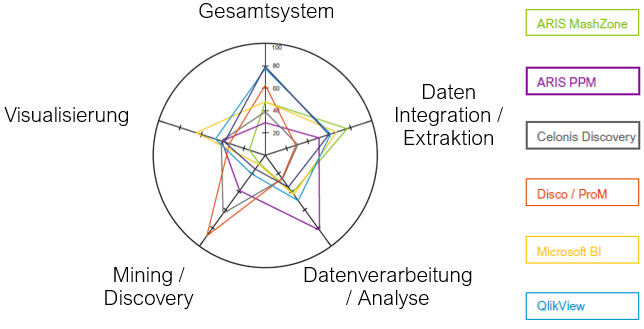
\includegraphics[scale=0.6]{figures/Appbildungen/toolEval.PNG}
    \caption{Bewertung von Process Mining Software (eigene Darstellung in Anlehnung an: J. Schobel, M. Reichert, 2017, S.244, \cite{Schobel2017})}
    \label{fig:toolEval}
\end{figure}

Neben der Bedienfreundlichkeit und dem Funktionsumfang sind die ausschlaggebenden Kriterien für die Auswahl der Software jene technische Daten, die sich direkt auf die praktische Umsetzbarkeit der Testreihe und des Proof of Concept auswirken. Die technischen Eckdaten wurden einer Abschlussarbeit mit dem Titel \textit{Vergleich und Evaluation von Process Mining Software} der Universität Passau entnommen \cite{compPM} und in Tabelle \ref{comparison2} zusammengefasst.

\begin{table}[!h]
\centering
\resizebox{\textwidth}{!}{%
\begin{tabular}{lccc}
\hline
Kriterium & \multicolumn{1}{c}{\textbf{ProM (V. 6.9)}} & \multicolumn{1}{c}{\textbf{Disco }} & \multicolumn{1}{c}{\textbf{Celonis}} \\
\hline\hline
\textit{Typ des Eingangslogs} & Mxml,xes & Csv,xls,XES,xml, fxl & Csv,Xls,XES \\
\textit{Process Discovery} & Ja & Ja & Ja \\
\textit{Lizenz} & Quelloffen & Kommerziell & Kommerziell \\
\textit{Notation der Ergebnisse} & BPMN, PNML, YAWL, PTML & XML & BPMN \\
\textit{Visualisierung der Prozesse} & Ja & Ja & Ja \\
\textit{lokale Anwendung} & Ja, Client-basiert & Ja, Client-basiert. & Nein, Cloud-basiert \\
\textit{Kommandozeilenanbindung} & Ja & Nein & Nein \\
\hline
\end{tabular}%
}
\caption{Gegenüberstellung von technischen Eigenschaften der populärsten Process Mining Lösungen (Quelle: Erling C., Vergleich und Evaluation von Process Mining Software, 2019, S. 36,37,44,83 [\ref{comparison2}])}
\label{comparison2}
\end{table}

Ein entscheidender Vorteil von ProM ist, dass einige der integrierten Plugins eine Kommandozeilenschnittstelle bieten. Mit Hilfe dieser kann die Auswertung der Eventlogs von einem serverseitigen Skript aus gestartet und überwacht werden. Nachteilig an dieser Lösung ist allerdings, dass ProM im Gegensatz zu Disco und Celonis Eventlogs im CSV-Format (\textit{Comma Seperated Values}) nicht direkt entgegen nimmt. Das bedeutet, dass eine Konvertierung in das XES Format stattfinden muss, bevor eine Process Mining Analyse durchgeführt werden kann.

Die quelloffene Lizensierung von ProM, die teils Cloud-basierte Architektur von Celonis und der Mangel einer Kommandozeilenanbindung von Disco sind ausschlaggebend für die Entscheidung, ProM als Werkzeug für die Durchführung des Process Mining in dieser Arbeit zu nutzen. 

\subsection{Wahl des Process Mining Algorithmus}
Es soll ein Process Mining Algorithmus identifiziert werden, der unter den in den Vergleich einbezogenen Minern am besten geeignet ist Modelle derart zu erzeugen, dass sie kurze, häufig auftretende Abläufe korrekt erkennen und abbilden. 

Mining Verfahren, deren Ausgabemodelle zwar korrekt, aber zu komplex sind um eine für den Anwender leicht interpretierbare Regel zu beschreiben sind für diesen Anwendungsfall ungeeignet. In Anbetracht der im Grundlagenkapitel erläuterten Gütekriterien (\ref{sec:quality}) werden hier Modelle gefordert, die ein hohes Maß an \textit{Simplicity} (Einfachheit) mitbringen und weniger Gewicht auf \textit{Generalization} legen, also kein Modell erstellen, das dazu neigt alle möglichen, selten auftretenden Prozesschritte mit einzubeziehen. 

Ein weiterer Faktor, der die Auswahl an Minern einschränkt, ist die praktische Umsetzbarkeit in einer realen Anwendung. Es werden nur solche Miner berücksichtigt, für die zum Zeitpunkt dieser Arbeit ein Plugin in der ProM-6.9-Version angeboten wird und die in der Lage sind, über Kommandozeilenbefehle so aufgerufen zu werden, dass sie direkt ein Ausgabemodell erzeugen. Das Ziel ist es einen automatisiert ablaufenden Dienst einzurichten, so dass Process Mining ohne zusätzliche Intervention seitens des Anwenders durchgeführt werden kann.

In ProM stehen Plugins des Heuristic, Local, Inductive und des Transitions System Miner zur Verfügung, die diese Anforderung erfüllen. Um beurteilen zu können, welches der Verfahren sich besonders für die Analyse von Eventlogs eignet, die menschliches Verhalten protokollieren, werden Veröffentlichungen herangezogen, die Process Mining im \textit{Activities of Daily Living} Kontext eingesetzt haben, sie sind in Tabelle \ref{tab:miningPaper} gelistet. 

Der Local Process Miner ist in der Tabelle nicht aufgeführt, da es bisher keine Veröffentlichungen gibt, die dieses noch junge Verfahren in einem vergleichbaren Kontext eingesetzt haben. 

\newcolumntype{b}{X}
\newcolumntype{s}{>{\hsize=.7\hsize}c}
\begin{table}[!ht]\small
\centering
\begin{tabularx}{\textwidth}{b ccc}
\hline
Titel                                                                                                               & \multicolumn{1}{l}{\textbf{Heuristic}} & \multicolumn{1}{l}{\textbf{Inductive}} & \multicolumn{1}{l}{\textbf{Transition}} \\ \hline\hline
\textit{Discovering process models of activities of daily living from sensors} \cite{adl1}                                      & x                                      &                                        &                                         \\
\textit{Context-based similarity measure on human behavior pattern analysis} \cite{adl2}                                        & x                                      &                                        &                                         \\
\textit{Mining insights from weakly-structured event data} \cite{adl3}                                                          & x                                      & x                                      &                                         \\
\textit{A novel human autonomy assessment system} \cite{adl4}                                                                   &                                        &                                        & x                                       \\
\textit{SAMDY–Technologies to support “Care On Demand”} \cite{adl5}                                                              &                                        &                                        & x                                       \\
\textit{Mining process model descriptions of daily life through event abstraction} \cite{adl6}                                  &                                        & x                                      &                                         \\
\textit{Recompiling learning processes from event logs} \cite{adl7}                                                             &                                        & x                                      &                                         \\
\textit{Event Abstraction for Process Mining Using Supervised Learning Techniques} \cite{adl8}                                  &                                        & x                                      &                                         \\
\textit{Visual process maps: a visualization tool for discovering habits in smart homes} \cite{adl9}                            &                                        & x                                      &                                         \\
\textit{Data Mining for Behavioural Changes and Monitoring Requirements in Residential} Healthcare \cite{adl10}                  & x                                      &                                        &                                         \\
\textit{Prozess-Mining und Prozessbewertung zur Verbesserung klinischer Workflows im Umfeld bilderzeugender Fächer} \cite{adl11} & x                                      &                                        &                                         \\ \hline

\end{tabularx}

\caption{Übersicht über Veröffentlichungen mit dem Thema Process Mining und ADL und das jeweils eingesetzte Process Mining Verfahren}
 \label{tab:miningPaper}
\end{table}
\normalsize
Betrachtet werden hier diejenigen Studien, die eines der Process Mining Algorithmen eingesetzt haben, für das ein Plugin in ProM 6.9 existiert, welches sich über eine Kommandozeilenanbindung ansprechen lässt. Ein weiteres Kriterium ist, dass in der Kurzfassung der Veröffentlichung die Absicht beschrieben wurde Protokolldaten, die menschliches Verhalten widerspiegeln, über Process Mining zu analysieren. Die Suche erfolgte über die Suchmaschine Google Scholar, die gesuchten Begriffe waren eine Kombination der Bezeichnung des jeweiligen Verfahrens und den Begriffen "ADL", "Smart Home", "Smart Living", "Human Activities" und "Human Behaviour". 

Es lässt sich ein eindeutiger Trend beobachten, der zeigt, dass sowohl der Heuristic als auch der Inductive Miner jeweils ein vergleichsweise populäres Mittel sind, um Protokolldateien, die menschliches Verhalten enthalten, auszuwerten, während der Transitions Miner weniger Beachtung findet. 

Zusätzlich sollen einige charakteristische Eigenschaften der Verfahren betrachtet werden, wie sie in Tabelle \ref{tab:my-table} aufgeführt sind. Sie ist angelehnt an einen Vergleich von Process Mining Algorithmen aus dem Buch \textit{Technisch unterstützte Pflege von Morgen} von M. Munstermann, erschienen 2015 im Springer Verlag \cite{munster}. Die Informationen zum Inductive und Local Process Miner sind den  Veröffentlichungen entnommen, die das jeweilige Verfahren vorstellen (Inductive \cite{inducIMining}, \cite{inducFMining}, Local \cite{localMining}). 

\begin{table}[!h]
\centering
\resizebox{\textwidth}{!}{%
\begin{tabular}{lcccc}
 Kriterien & \textbf{Heuristic} & \textbf{Transition} & \textbf{Inductive} & \textbf{Local}   \\
%Betrachtete Plugin Version & F. Mannhardt, Interactive Data Aware Heur. M. & H.M.W. Verbeek, Mine for a fuzzy Model & S.J.Leemans, Mine with Inductive Visual Miner & N.Tax, Search for Local Process Models \\
\hline\hline
Nebenläufigkeit & + & + & + & + \\
kurze Iterationen (Schleifenlänge ≤ 2) & + & + & + & + \\
Eignung für unvollständige &  &  &  &  \\
Eventlogs & + & + & + & + \\
Eignung für fehlerbehaftete &  &  &  &  \\
Eventlogs & + & - & + & - \\
Frequenz von Traces &  &  &  &  \\
wird berücksichtigt & + & - & + & + \\
automatisierbar & + & + & + & +\\
\hline
\end{tabular}%
}
\caption{Eigenschaften von Process Mining Verfahren zur Beurteilung ihrer Eignung für den Einsatz im Smart Home (Quelle: M.Munstermann, Technisch unterstützte Pflege von morgen, 2015, S.101 \cite{munster}}
\label{tab:my-table}
\end{table}
Ein + symbolisiert, dass ein Kriterium erfüllt wird, ein - kennzeichnet, dass das Kriterium nicht erfüllt wird. Aus dieser Tabelle geht hervor, dass sowohl der Inductive als auch der Heuristic Miner über Strategien verfügen, um komplex gestaltete Eventlogs zu verarbeiten. 

Diese Eigenschaften sowie die Tendenz in der Forschung, den Inductive Miner und Heuristic Miner in Smart Home ähnlichen Szenarien einzusetzen, wie in Tabelle \ref{tab:miningPaper} zu erkennen ist, wurde als hinreichende Bewertungsgrundlage angenommen, um den Heuristic Miner und den Inductive Miner auszuwählen, um sie in einer Testreihe einem Vergleich zu unterziehen. 

\subsection{Generieren von Protokolldateien}
Um zu untersuchen, inwieweit die Ausgabemodelle der gewählten Miner sich für den im Rahmen dieser Arbeit geplanten Anwendungsfall eignen, werden Eventlogs benötigt, die menschliches Verhalten protokollieren, welches kurze und regelmäßige Abläufe enthält. Mangels einer realen Smart Home Datenquelle werden die Protokolldateien durch ein im Rahmen dieser Arbeit entstandenes Python Programm generiert, das im Anhang zu einzusehen ist \ref{lst:generate}.

Aufgrund der nahezu unbegrenzten Anzahl möglicher Szenarien, die in einem Smart Home durch Protokolldateien aufgenommen werden könnten, kann hier nur ein Ausschnitt simuliert werden. Um dennoch eine hohe Aussagekraft der Testreihe zu erhalten, werden die Eventlogs derart gestaltet, dass sie gegenüber dem Miner inkrementell komplexer werden und so Performanzunterschiede zwischen den Algorithmen sichtbar werden können. 

Hervorzuheben ist an dieser Stelle, dass die Miner den Inhalt einzelner Einträge nicht deuten, sie unterscheiden die Ressourcen, die den Eintrag erstellt und die zugehörigen Attribute nur Anhand der Zeichenkette im Protokoll. Dementsprechend werden die Namen der IoT Ressourcen und ihre Aktivitäten hier zwar beispielhaft für gängige vernetzte Geräte gewählt, sie haben jedoch keinen direkten Einfluss auf das Ergebnis des Mining Verfahrens und sind beliebig austauschbar. Signifikant für die Auswertung ist zunächst nur die Häufigkeit, mit der eine Ressource einen Eintrag erstellt, und der Zeitpunkt des Eintrags im Protokoll, der zu dieser Ressource gehört.

Um die generierten Protokolldateien strukturell nah an realistischen Protokolldateien zu gestalten, wurden sie um Rauscheinträge durch die Funktion addnoise() ergänzt. In einer realen Smart Home Umgebung ist es wahrscheinlich, dass nicht nur kurze Routinen der Bewohner aufgezeichnet werden, sondern auch für Regeln irrelevante Sensoraufnahmen erscheinen, oder Aktivitäten die nicht Teil einer Routine sind.

Einr generierte Protokolldatei wird also durch drei Faktoren definiert: das eingebettete, vom Miner zu erkennende Verhaltensmuster, die Menge an konsekutiven Kalendertagen (30 o. 90 Tage), die der Länge der Aufnahmezeit entspricht und den Anteil an Rauscheinträgen (jeweils 15 oder 50 pro Tag). Eine erfolgreiche Auswertung durch einen Miner hat stattgefunden, wenn das in der Protokolldatei eingebettete Muster vollständig im Modell wiedergegeben wird, parallele Abläufe korrekt dargestellt werden und keine überschüssigen (Rausch-) Einträge als Knoten im Ausgabemodell enthalten sind.

Die Testreihe setzt sich aus zwölf verschiedenen Mustern zusammen. Da für jedes gesuchte Muster jeweils vier Protokolldateien generiert wurden (mit 30 oder 90 Tagen, mit einem Rauschanteil von je 15 oder 50 Einträgen), entstehen insgesamt 48 Protokolldateien, die Aufnahmen aus einem Smart Home simulieren. Die Testreihen tragen jeweils die Namen der Muster (genannt „A“ - „M“), insgesamt sind 104 einzelne Wenn-Dann Regeln in den Mustern enthalten. Pro Testreihe sind maximal vier und mindestens eine Regel eingebettet. Die Regeln sind in einer Übersicht im Anhang \ref{sec:config} einsehbar. 

\section{Bewertungskriterien und Durchführung der Testreihe}\label{sec:tests}
Die Durchführung der Testreihe bestand darin jedes der zuvor generierten Eventlogs mit dem Heuristics Miner und dem Inductive Miner auszuführen und das Ergebnis zu protokollieren. 

Um die Güte der Modelle, die in der Messreihe mit den verschiedenen Minern entstanden sind, zu evaluieren, wurden die Ausgabemodelle der Process Mining Plugins mit dem ursprünglich eingebetteten Modell verglichen und der Grad der Abweichung für jeden Datensatz dokumentiert. Um die Performanz der Miner zu quantifizieren, wird die Wiedergabe der eingebetteten Muster im Ausgabemodell über ein Punktesystem bewertet. 

Entscheidend für den im Rahmen dieser Arbeit betrachteten Anwendungsfall der automatisierten Regelerkennung im Smart Home ist, dass der Mining Algorithmus in der Lage ist, Rauschen aus dem Modell herauszufiltern und korrekt kurze Pfade und sowie ihre Parallelität zu identifizieren. Für jedes Ausgabemodell wird die Anzahl der korrekt erkannten Regeln (\textit{True Positive}) gezählt. Wenn keine überschüssigen Einträge im Modell erscheinen  (\textit{False Postive}) und keine für Regeln relevante Einträge fehlen (\textit{False Negative}) wird ein Punkt verteilt, andernfalls null Punkte notiert. 
Desweiteren sind Ausgabemodelle nur dann für die Weiterverarbeitung verwertbar, wenn die Einträge, die zu unterschiedlichen Regeln gehören, auch auf unterschiedlichen Pfaden im Modell abgebildet werden. Als weitere Metrik in der Testreihe wird daher die Anzahl der korrekt erkannten Pfade im Ausgangsmodell verwendet (\textit{Parallelism}). Wenn das Ausgabemodell mit dem eingebetteten Muster einer Protokolldatei übereinstimmt, erhält der Miner die volle Punktzahl für das jeweilige Ausgabemodell. 

\section{Auswertung der Ergebnisse}\label{sec:res}
Aus der Dokumentation der Testreihe geht hervor, dass es signifikante Unterschiede in der Fähigkeit der untersuchten Mining Algorithmen gibt, Abläufe mit vielen kurzen Pfaden zu identifizieren und im Ausgabemodell korrekt wiederzugeben. Lediglich für fünf der zwölf Reihen geben beide Miner das gesuchte Resultat fehlerfrei aus (konkret: A,B,D,E,F), siehe Tabelle\ref{tab1} und Tabelle \ref{tab2} im Anhang. 

In den sieben Reihen, in denen einer der beiden Miner Plugins fehlerhafte Ausgabemodelle produzierte, handelte es sich in fünf Fällen (H,J,K,L,M) um das ‚Inductive Visual Miner Plugin‘. Dahingegen ergaben sich beim ‚Interactive Data-aware Heuristics Miner‘ Plugin lediglich in zwei Testreihen (C,G) unbrauchbare Ausgabemodelle. Die Auswertung der Testreihe hat auch gezeigt, dass beide Miner gut geeignet sind bis zu zwei Regeln in einem Eventlog zu erkennen. Bei regelmäßigem Auftreten der Regel konnten auch kurze Auswertungszeitspannen und ein hohes Maß an Rauscheinträgen das Ausgabemodell nicht verzerren.

Im Unterschied zum Heuristic Miner Plugin gelang es dem Inductive Miner Plugin nicht, mehr als zwei kurze Regeln, die in die Eventlogs der Testreihen H,J,K,L,M eingebettet waren, korrekt in parallel verlaufende Pfaden zu unterteilen. Stattdessen gab der Miner häufig alle gesuchten Elemente auf einem einzigen Pfad des Petri Netzes aus, wie es auf Abbildung \ref{fig:H_inductive} zu sehen ist. 

Es gelang ihm nicht, die Parallelität der gesuchten Abläufe zu abzubilden. 


\begin{figure}[!ht]
    \centering
    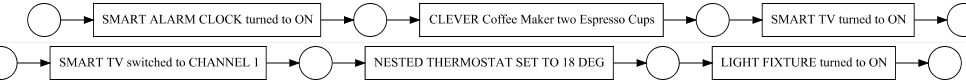
\includegraphics[width=\textwidth,]{figures/Appbildungen/H_induct.PNG}
    \caption{Modellierung einer Protokolldatei der Testreihe H mit dem Inductive Miner Plugin}
    \label{fig:H_inductive}
\end{figure}

Ein Ausgebemodell des Heuristic Miners, das für das gegebene Eventlog alle Regeln korrekt abstrahiert, ist auf Abbildung \ref{fig:H_heurist} zu sehen.


\begin{figure}[!ht]
    \centering
    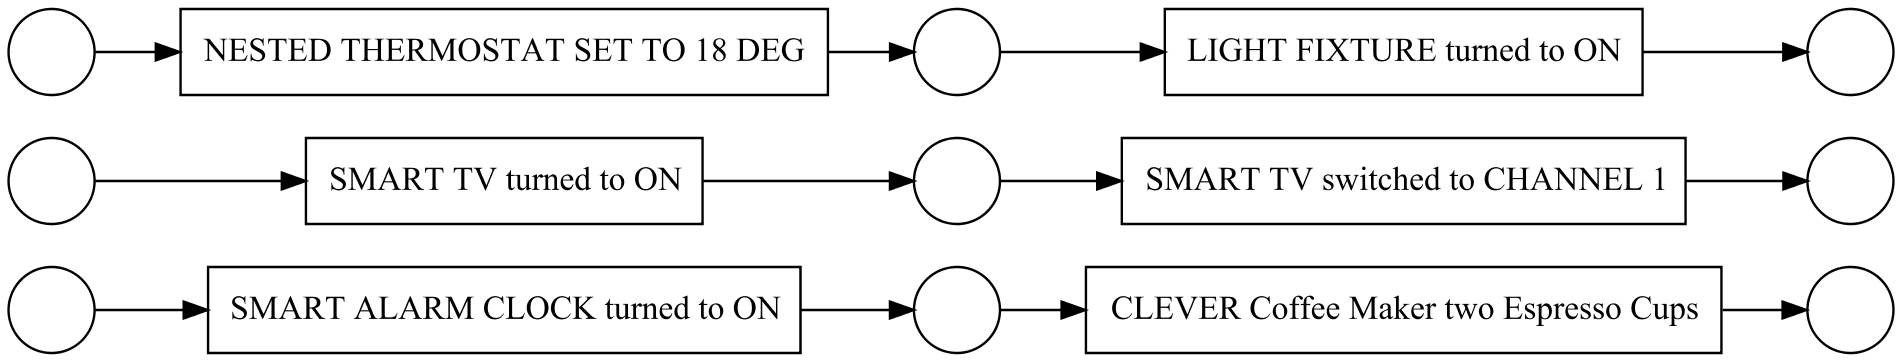
\includegraphics[width=0.95\textwidth,]{figures/Appbildungen/H_heurist.PNG}
    \caption{Modellierung einer Protokolldatei der Testreihe H mit dem Heuristic Miner Plugin}
    \label{fig:H_heurist}
\end{figure}

Aus der Perspektive des Inductive Miner Verfahrens betrachtet lies sich also beobachten, dass es an dieser hier nicht gelang, einen \textit{XOR Cut}, wie in  \ref{sec:inducMiner} beschrieben, an der Stelle zu setzen, an der mehr als zwei kurze parallele Abläufe beginnen. 

Beispielhaft für eine andere Abweichung von der gesuchten Modellierung kann ein Modell der Reihe 'K' betrachtet werden. Eingebettet in die hier eingesetzten Eventlogs lagen drei separate, regelmäßig auftretende Wenn-Dann Abfolgen, bestehend aus jeweils zwei oder drei Elementen. 
Für alle vier Kombinationsmöglichkeiten zur Konfiguration des Eventlogs (30 Tage simulierter Aufnahmezeitraum mit einem Rauschanteil von 15 oder 50 Einträgen und ein Zeitraum von  90 Tagen mit einem Rauschanteil von 15 oder 50) berechnete der Heuristic Miner ein Modell, welches die drei erwarteten Abfolgen enthielt und alle Rauscheinträge herausfiltern konnte, wie in Abbildung \ref{fig:K_heuristic} zu sehen ist.
\begin{figure}[!h]
    \centering
    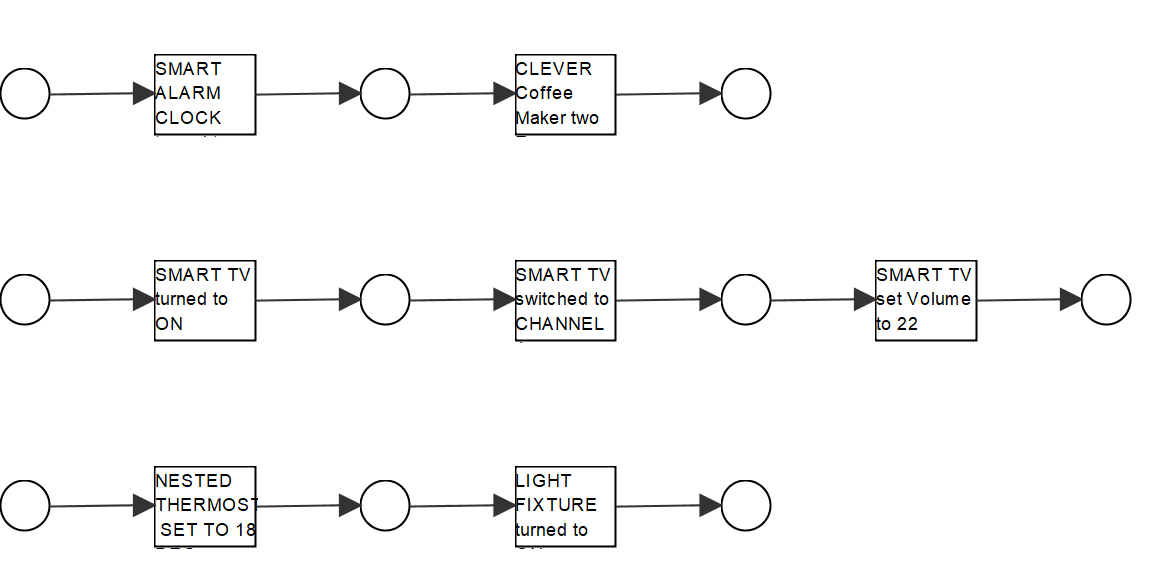
\includegraphics[width=0.8\textwidth,]{figures/Appbildungen/K_heuristic_correct.PNG}
    \caption{Modellierung einer Protokolldatei der Testreihe K mit dem Heuristic Miner Plugin}
    \label{fig:K_heuristic}
\end{figure}
\newpage
Auch das Inductive Miner Plugin war in der Lage das Rauschen herauszufiltern, modellierte aber, bei Eingabe der selben Eventlog Dateien, die das Heuristic Miner Plugin genutzt hat, ein für den Einsatzzweck ungeeignetes Modell. 

Auf Abbildung \ref{fig:K_inductive} ist zu sehen, dass nur eine Regel korrekt in der Wenn-Dann Folge abgebildet wird: auf eine 'Smart Alarm Clock' Aktivität folgt eine 'Coffee Maker' Aktivität. 

\begin{figure}[!h]
    \centering
    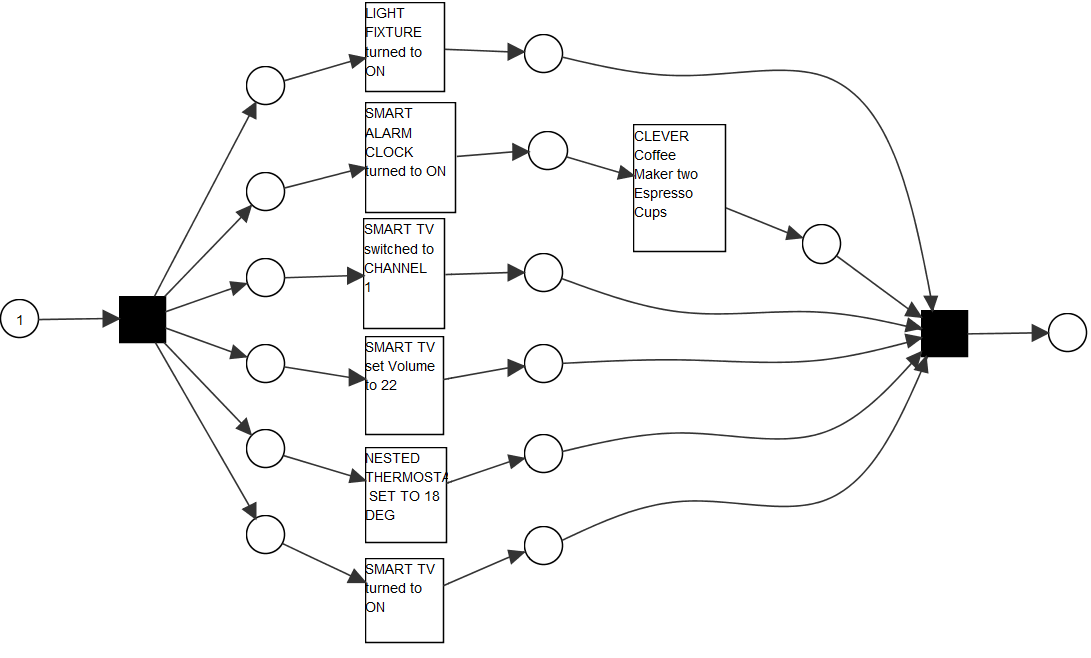
\includegraphics[width=0.8\textwidth,]{figures/Appbildungen/K_inductive_erronousPNG.PNG}
    \caption{Modellierung einer Protokolldatei der Testreihe K mit dem Heuristic Miner Plugin}
    \label{fig:K_inductive}
\end{figure}

Die Komponenten der restlichen eingebetteten Regeln werden zwar erkannt, aber nicht in der korrekten Abfolge, sondern parallel zueinander abgebildet. Diese Form der Abweichung hat sich als charakteristisch für den Inductive Miner herausgestellt. Auch die resultierenden Modelle des Inductive Miner der Reihen H,J,L,M enthielten zwar häufig die gesuchten Einträge, allerdings nicht in der gewünschten Reihenfolge. Es entstanden teilweise sogenannte Blumenmodelle, wie sie eingangs beschrieben wurden, siehe Abschnitt \ref{sec:quality}. Die Modellierung fiel also zu allgemein aus, als dass sie gebraucht werden könnte, um in ein If This Then That Schema überführt zu werden.

Auch der Heuristic Miner generierte nicht für jedes Eventlog das erwartete Modell, beispielsweise gelang es ihm in der Testreihe C nicht, alle zur Regel gehörenden Einträge zu erkennen. Es fehlt ein weiterer Eintrag auf dem ersten Pfad. Die erkannten Einträge wurden jedoch korrekt angeordnet, siehe Abbildung \ref{fig:C_heuristic}. 

\begin{figure}[!ht]
    \centering
    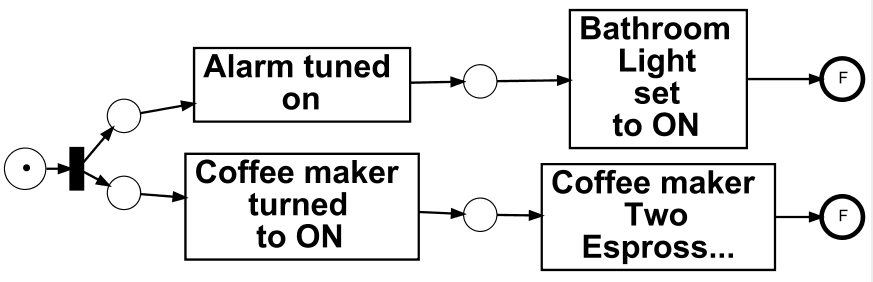
\includegraphics[width=0.6\textwidth,]{figures/Appbildungen/C_Heuristic.PNG}
    \caption{Modellierung einer Protokolldatei der Testreihe C aus dem Heuristic Miner Plugin}
    \label{fig:C_heuristic}
\end{figure}

Aus der Auswertung der Testreihe geht hervor, dass aus insgesamt 104 Regeln, die in den 48 Eventlogs eingebettet wurden, der Heuristic Miner 96 korrekt identifiziert hat, der Inductive Miner hingegen nur in 48 Fällen die gesuchten Regeln korrekt abbilden konnte.

\begin{table}[!htbp]
\centering
\resizebox{\textwidth}{!}{%
\begin{tabular}{l|ccccc}
Algorithmus                & \multicolumn{1}{l}{\textbf{Testreihen}} & \multicolumn{1}{l}{\textbf{Regeln}} & \multicolumn{1}{l}{\textbf{Fehlerhafte Modelle}} & \multicolumn{1}{l}{\textbf{Identifizierte Regeln}} & \multicolumn{1}{l}{\textbf{Verfehlte Regeln}} \\ \hline
\textit{Inductive M.}  & 48                                      & 104                                 & 14                                               & 48                                                 & 56                                            \\
\textit{Heuristics M.} & 48                                      & 104                                 & 2                                                & 96                                                 & 8                                            
\end{tabular}%
}
\caption{Ergebnisse der Auswertung der Versuchsreihe}
\label{tab:results_short}
\end{table}

Da ein Verfahren gesucht wurde, das kurze Regeln, also Abläufe bestehend aus zwei bis vier Elementen, erkennt und in der Lage ist mehrere Regeln, die in einem Eventlog eingebettet sind klar voneinander zu trennen, ging das Heuristic Miner Plugin aus der hier vorgestellten Testreihe als zu bevorzugendes Verfahren hervor.

Neben den Erkenntnissen über die wahrscheinliche Eignung der untersuchten Process Mining Verfahren für den Einsatz zur automatisierten Regelerkennung, konnte außerdem beobachtet werden, welche Parameter, die den Process Mining Verfahren eigen sind, eine positive oder negative Auswirkung auf die Auswertung haben. 

So gibt es beispielsweise die Möglichkeit, in der Konfiguration des Heuristic Miner Plugin "all tasks connected", also "Verbinde alle Abläufe" auf \textit{wahr} zu setzen, was konsistent zu Modellen führt, die von Anwendern und Entwicklern des Process Mining gemeinhin als ,Spaghettimodell' bezeichnet werden, wie es hier für einen Datensatz der Testreihe A in Abbildung \ref{fig:A_heuristic_spagh} zu sehen ist.
\begin{figure}[!ht]
    \centering
    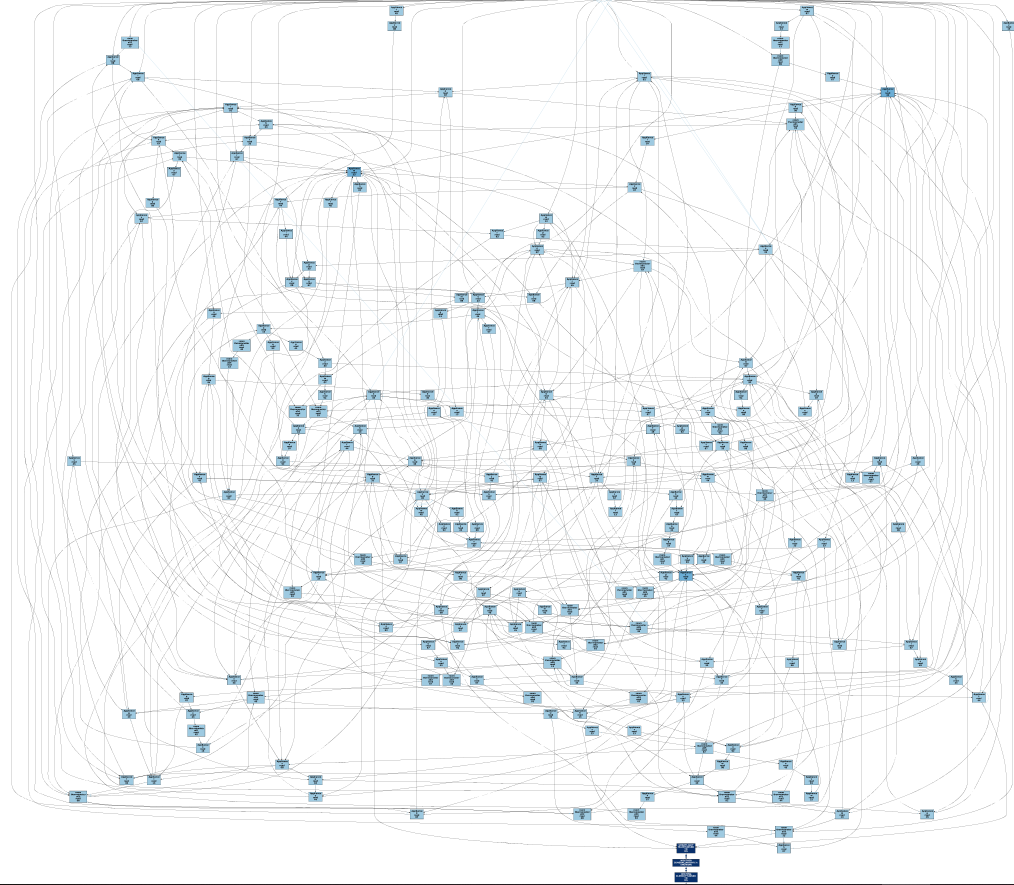
\includegraphics[width=0.65\textwidth,]{figures/Appbildungen/A_underfitted.PNG}
    \caption{Modellierung einer Protokolldatei der Testreihe A aus dem Heuristic Miner Plugin}
    \label{fig:A_heuristic_spagh}
\end{figure}

Basierend auf den Erkenntnissen dieser Testreihe wurde das Heuristic Miner Plugin gewählt, um ihn für die Konstruktion des Proof of Concept einzusetzen und desweiteren notiert, dass der Parameter "all tasks connected" auf \textit{false} zu setzen ist.
%Desweiteren deutet die Auswertung der Testreihe darauf hin, dass der Einsatz des Heuristic Miners möglicherweise Prinzipiell gegenüber dem Inductive Miner zu bevorzugen ist, wenn nach einer Modellierung gesucht wird, die dem If This Then That Schema entspricht, also Muster enthält, die jeweils aus mehreren Ketten besttenur wenigen aufeinanderfolgenden Elementen bestehen.





%\Rotatebox{90}{%
%\centering
%    \begin{tabular}{lp{2cm}p{2cm}p{2cm}p{2cm}p{2cm}p{2cm}}
%& Alpha Miner & Heuristic Miner & Heuristic Miner + & Fuzzy %Miner & Transition System Miner & Transition System Miner + %\\
%(garantierte) Ausführbarkeit & - & ? & ? & - & + & + \\
%Nebenläufigkeit & + & + & + & - & + & + \\
%Intervalle & - & - & + & - & + & + \\
%kurze Iterationen (Schleifenlänge ≤ 2) & - & + & + & + & + & %+ \\
%entfernte Abhängigkeiten/ nicht lokales Verhalten & - & + & + %& + & + & + \\
%nicht wahrnehmbare Aktivitäten & - & + & + & - & + & + \\
%Eignung für unvollständige Event Logs & - & + & + & + & + & + %\\
%Eignung für fehlerbehaftete Event Logs & - & + & + & + & - & %- \\
%Frequenz von Traces wird berücksichtigt & - & + & + & ? & - & %+ \\
%parametrisierbar & - & + & + & + & + & + \\
%automatisierbar & + & - & - & - & - & + \\
%tolerant gegenüber unstrukturierten Prozessen & - & ? & ? & + %& - & - \\
%ein Mining-Schritt & + & + & + & + & - & - \\
%zwei Mining-Schritte & - & - & - & - & + & + \\
%Ausgabeformat & & & & & & \\
%Petri-Netz & + & - & - & - & + & + \\
%heuristisches Netz & - & + & + & - & - & - \\
%Fuzzy-Modell & - & - & - & + & - & - \\
%Transitionssystem & - & - & - & - & + & + \\
%\end{tabular} 
%}

%\begin{table}[h!]
%\centering
%\begin{tabular}{ccccccc}
%& Alpha Miner & Heuristic Miner & Heuristic Miner + & Fuzzy Miner & Transition System Miner %& Transition System Miner + \\
%(garantierte) Ausführbarkeit & - & ? & ? & - & + & + \\
%Nebenläufigkeit & + & + & + & - & + & + \\
%Intervalle & - & - & + & - & + & + \\
%kurze Iterationen (Schleifenlänge ≤ 2) & - & + & + & + & + & + \\
%entfernte Abhängigkeiten/ nicht lokales Verhalten & - & + & + & + & + & + \\
%nicht wahrnehmbare Aktivitäten & - & + & + & - & + & + \\
%Eignung für unvollständige Event Logs & - & + & + & + & + & + \\
%Eignung für fehlerbehaftete Event Logs & - & + & + & + & - & - \\
%Frequenz von Traces wird berücksichtigt & - & + & + & ? & - & + \\
%parametrisierbar & - & + & + & + & + & + \\
%automatisierbar & + & - & - & - & - & + \\
%tolerant gegenüber unstrukturierten Prozessen & - & ? & ? & + & - & - \\
%ein Mining-Schritt & + & + & + & + & - & - \\
%zwei Mining-Schritte & - & - & - & - & + & + \\
%Ausgabeformat & & & & & & \\
%Petri-Netz & + & - & - & - & + & + \\
%heuristisches Netz & - & + & + & - & - & - \\
%Fuzzy-Modell & - & - & - & + & - & - \\
%Transitionssystem & - & - & - & - & + & + \\
%\end{tabular} 
%\caption{Eigenschaften der wichtigsten Mining Algorithmen}
%\label{table:1}
%\end{table}